\documentclass[german,a4paper,12pt]{llncs}
\setcounter{tocdepth}{2}
\makeatletter
\renewcommand*\l@author[2]{}
\renewcommand*\l@author[2]{}
\makeatletter
\usepackage[utf8]{inputenc}
\usepackage[backend=biber,sorting =none]{biblatex}
\usepackage{csquotes}
\usepackage{graphicx}
\usepackage{babel}

\usepackage{parskip}
\usepackage{float}

%\usepackage{hyperref}
\usepackage{filecontents}


\begin{filecontents}{references.bib}
	
@article{visualScale,
	author = {Martínez-Velasco, María and Vázquez-Herrera, Norma and Maddy, Austin and Asz-Sigall, Daniel and Tosti, Antonella},
	year = {2017},
	month = {02},
	pages = {},
	title = {The Hair Shedding Visual Scale: A Quick Tool to Assess Hair Loss in Women},
	volume = {7},
	journal = {Dermatology and Therapy},
	doi = {10.1007/s13555-017-0171-8}
}

@inproceedings{GreenScreenHair,
	author = {Legendre, Chloe and Krissman, David and Debevec, Paul},
	year = {2017},
	month = {07},
	pages = {1-2},
	title = {Improved chromakey of hair strands via orientation filter convolution},
	isbn = {978-1-4503-5015-0},
	doi = {10.1145/3102163.3102200}
}
@article{seasoalShedding,
	
	author = {Hsiang, E.Y. and Semenov, Yevgeniy and Aguh, Crystal and Kwatra, S.G.},
	year = {2017},
	month = {10},
	pages = {},
	title = {Seasonality of hair loss: a time series analysis of Google Trends data 2004 to 2016},
	volume = {178},
	journal = {British Journal of Dermatology},
	doi = {10.1111/bjd.16075}
}

@inbook{chemicalAlopecia,
	author = {Maibach, Howard and Yamaguchi, Ian},
	year = {2012},
	month = {01},
	pages = {1935-1942},
	title = {Chemically Induced Hair Loss/Alopecia},
	isbn = {978-3-642-02034-6},
	journal = {Kanerva's Occupational Dermatology, Second Edition},
	doi = {10.1007/978-3-642-02035-3_205}
}

@article{ironDeficiency,
	author = {Trost, Leonid and Bergfeld, Wilma and Calogeras, Ellen},
	year = {2006},
	month = {06},
	pages = {824-44},
	title = {The diagnosis and treatment of iron deficiency and its potential relationship to hair loss},
	volume = {54},
	journal = {Journal of the American Academy of Dermatology},
	doi = {10.1016/j.jaad.2005.11.1104}
}

https://matplotlib.org/
https://numpy.org/

\end{filecontents}

\addbibresource{references.bib}
\title{Exposee}
\subtitle{Automatisches Schätzen der Haaranzahl in ausgefallenen Haarbüscheln}
\author{\parbox{.9\textwidth}{\centering 
		\large Janelle Pfeifer \\
		\small Delpstraße 28\\
		53359 Rheinbach \\
		janelle.pfeifer@smail.inf.h-brs.de}}
\institute{\parbox{.9\textwidth}{\centering 
		\large Hochschule Bonn-Rhein-Sieg \\
		\normalsize Institute of Visual Computing \\ 
		\small Fachbereich Informatik \\
		Studiengang: Informatik (B.SC.)\\
		\normalsize Rheinbach, 15.02.2020}}
\date{Rheinbach, 8.1.2020}
\begin{document}
	%{\let\newpage\relax\maketitle}
	\maketitle
	\newpage
	\tableofcontents
	\newpage

\begin{abstract}
	am ende hier ein abstract hin
\end{abstract}

\section{Einleitung}
Die Einleitung ist mit der wichtigste Teil der Arbeit, da sie den Leser motivieren soll die vorliegende Arbeit weiter z lesen. Sie sollte neben einer Motivation bzw Problembeschreibung auch das Ziel der Arbeit beschreiben.Zusätzlich sollten die Fabgebiete die die arbeit betreffen und deren Bedeutung genannt werden. Wichtig ist eine klare Formulierung der Zielstellung und des Lösungsansatzes so wie abschließend eine Beschreibung der Gliederung der Arbeit.

Das Ausfallen von Haarsträhnen ist ein natürlicher Teil des Haarwachstum Zyklus. Durchschnittlich verliert 50 bis 100 Haarsträhnen am Tag. Vermehrter Haarverlust kann ein Indikator von Krankheit oder anderen Problemen sein. Da ist es von Vorteil das früher zu erfahren.

Der Haarverlust wird von unterschielidchen faktoren beeinflusst. So gibt es seasonale unterschiede. Haartextur und länge verändert den eindruck den eine person. so ist es nicht leicht den normalen haarverlust für eine person festzustellen 

computer vision. was ist das?

das paper gibt einstig in haar estimation mit computer vision. In dem Paper \blockquote{The Hair shedding visual scale: A quick tool to assess hair loss in Women} wird eine Methode beschrieben, in der Frauen anhand von Bildern den Umfang ihres täglichen Haarausfalls bestimmen können. Dabei werden den Frauen Bilder von abgezählten, ausgefallenen Haarbüscheln gezeigt, die ihrer eigenen Haarlänge entsprechen. Die Frauen wählen das Foto aus, welches ihrem persönlichen täglichen Haarausfall entspricht. Es wurde eine Korrelation festgestellt zwischen Frauen, die klinisch bestätigt Haarverlust erfahren und den Bildern, die sie ausgewählt haben.\cite{visualScale}

In dieser Arbeit wird ein verfahren vorgestellt mit dem eine langzeitüberwachung des täglichen Haarverlustes duchgeführt werden kann.

\section{Grundlagen}

\section{Design}

Das Ziel ist es die Einschätzung eines Haarbüschels, mithilfe von Computervision, zu automatisieren. Es soll ein Kalibriervorgang geben, in dem der Nutzer abgezählte Haarbüschel-Bilder eingibt. Nach der Kalibrierung soll die Menge der Haare in nicht abgezählten Haarbüscheln automatisch geschätzt werden.

Die Schätzungen werden zugehörig zum Datum gespeichert. 
Zusätzlich zu den Schätzungen können für jedes Datum eine Marker angegeben werden, das regelmäßige Wiederholungen der Haarpflege, wie zum Beispiel eine Haarwäsche, notiert.

So wird eine Langzeitüberwachung der Menge des Haarausfalls möglichst detailliert und mit geringem Arbeitsaufwand für einen menschlichen Nutzer durchführbar.

detection

gessfunctions
Daten aus Bildern ziehen. In einem Calibrationsschritt daten aus mehreren unterschieldichen bildern nehmen und mithilfe von vordefinierten parametern korrelation zwischen haarmenge und daten zu finden.

Calibration genauer. was wird da gemacht ? assume alle fachbegriffe und algorithmen sind bekannt.
guess genauer. guessfunctions. 
beschreibe das gespeichert wird
beschreibe das es ein kommandozeilenprogramm ist
mehrere user
\section{Bildverarbeitung}

Mithilfe von Methoden der Bildverarbeitung wird eine Reihe an Daten über eingegebene Haarbüschel Bilder extrahiert.
Dieser Schritt ist in der Methode detect implementiert.
Als Eingabe wird von einem Haarbüschel auf einem einfarbige Hintergrund ausgegangen. Dabei sollte ein möglichst guter Kontrast zu der Haarfarbe gewählt worden sein. Beispielsweise ein weißer Hintergrund für dunkele haare oder ein schwarzer Hintergrund für blondes oder hellbraunes Haar. Die Ecken des Hintergrundes sind durch ein Symbol markiert. Vergleich Abbildung \ref{img:input}.

\begin{figure}
	\centering
	
\includegraphics[width=0.9\textwidth]{fig64/00IMG_20200406_153354_12_g_15.jpg}
	\caption[]{Input}
	\label{img:input}
\end{figure}

Im ersten schritt der Bildverarbeitung wird das Bild auf die Markierungen in den Ecken zugeschnitten. Das ist in der Methode cropDots implementiert.
Über einen Aufruf der open cv methode matchTemplate wird nach vorkommen der Markierung zu suchen. Das Resultat ist ein Karte an Wahrscheinlichkeiten die für jedes Pixel angibt, zu welchen Wahrscheinlichkeit sich dort die Markierung befindet. Die 4 Stellen an denen die Wahrscheinlichkeit am höchsten ist, werden als Eckpunkte angesehen. 

\begin{figure}
	\centering
	
\includegraphics[width=0.9\textwidth]{fig64/01match res.png}
	\caption[]{Resultat von matchTemplate}
	\label{img:matchTempate}
\end{figure}

\begin{figure}
	\centering
	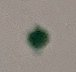
\includegraphics[width=0.2\textwidth]{fig64/TemplateDot.jpg}
	\caption[]{Das Aussehen der Markierung ist bekannt und wird über so ein Bild angegeben.}
	\label{img:TemplateDot}
\end{figure}

\begin{figure}
	\centering
	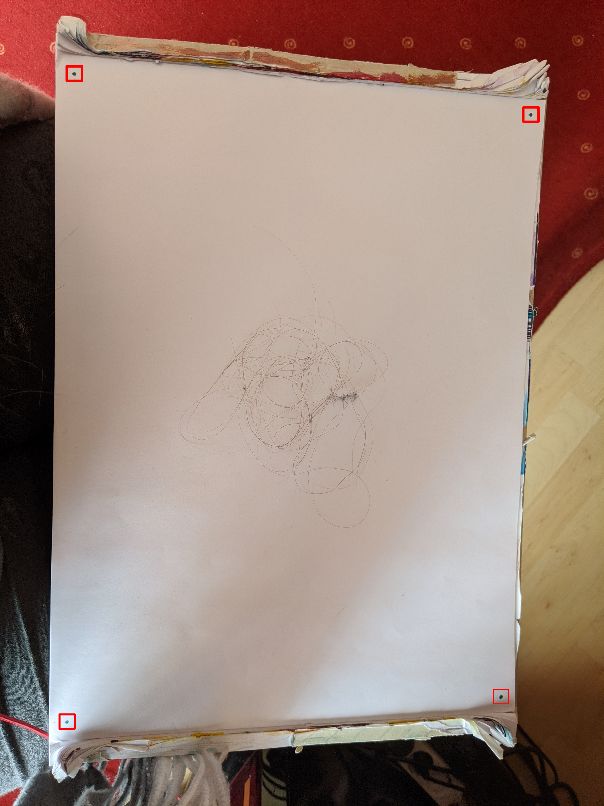
\includegraphics[width=0.9\textwidth]{fig64/03rectImg.png}
	\caption[]{Die 4 erkannten Markierungen im Bild}
	\label{img:foundDots}
\end{figure}
\begin{figure}
	\centering
	
\includegraphics[width=0.9\textwidth]{fig64/03crop image.png}
	\caption[]{Resultat des Zuschneidens}
	\label{img:Crop}
\end{figure}

Durch das Zuschneiden der Bilder wird sichergestellt, das die Haare immer etwa einen gleich großen Hintergrund haben. So werden die Daten die aus den Bildern gezogen werden nicht verfälscht dadurch, das die Haare eventuell von unterschiedlichen Abständen fotografiert wurden. 

Nach dem Zuschneiden werde die Haare von dem Hintergund getrennt.
Das ist in der Methode edgeProcess implementiert.




\section{Implementation}

mit python
nutzt plugin open cv und plugins ....

\subsection{Daten aus Bildern ziehen.}
der vorgang davon...
\subsection{Calibrierung}
calibrierung
ganzen ornder kalibrieren. einzelne bilder hinzufügen.
\subsection{guess}





\subsection{Haarausfall}
Wie in dem Paper \blockquote{The Hair shedding visual scale: A quick tool to assess hair loss in Women} beschrieben, kann man den täglichen Haarausfall als Indikation des gesamten Haarausfalls nehmen.\cite{visualScale}

Haarausfall wird von mehrere Faktoren bestimmt und ist grundlegend gesund. Haarausfall ist nicht uniform. Er kann sich abhängig von dem Haartyp, der Haarlänge und der Haarpflege-Methode jeden Tag ändern und Muster aufweisen. 

Eine Person die ihre Haare einmal in der Woche kämmt kann zum Zeitpunkt des Kämmens mehr Haarausfall erwarten, als eine Person die ihre Haare jeden Tag kämmt. 

Hinzukommen saisonale Unterschiede in dem Haarverlust.\cite{seasoalShedding}

Jeder Mensch hat ein eigenes Haarausfall-Muster. Abweichungen von diesem Muster können Anzeichen von Krankheiten und Mangelerscheinungen sein. Beispielsweise ist erhöhter Haarausfall ein Symptom von Eisenmangel.\cite{ironDeficiency}

\subsection{Computervision}
In dem Bereich der Bildverarbeitung gibt es viele Algorithmen, die es ermöglichen Objekte in einem Bild erkennbar zu machen und zu verarbeiten.

\subsubsection{Region Growth}
ist ein Verfahren, bei dem ein Bild in Regionen unterteilt wird. So werden zum Beispiel Sektionen mit ähnlicher Farbe herausgestellt. 

\subsubsection{Skelettierung}
reduziert Objekte in einem Bild auf eine Pixelbreite. So können Linien auf eine Pixelbreite geschrumpft werden.

\subsubsection{Dynamischer Schwellwert}
kann genutzt werden, um Schatten aus einem Bild zu entfernen. Ein dynamischer Schwellwert ist geeignet für kompliziertere Bildern und Belichtungssituationen.


\subsubsection{Hochpassfilter}
erhält hochfrequente Bildanteile, während Niederfrequente verschwindet bzw. abgeschwächt werden. 
Hochfrequent sind Bereiche mit schnellen Farb- und Helligkeitsveränderungen. Das tritt beispielsweise bei Linien und Kanten auf.

\subsubsection{Kantendetektion}

nutzt Hochpassfilter, um Kanten in einem Bild zu erkennen. 

\subsection{Erkennung von Haaren in Green-Screen Bildern}

In dem Paper\blockquote{Improved Chromakey of Hair Strands via Orientation Filter Convolution} wird eine Methode beschrieben wie Haarsträhnen von einem Green-Screen Hintergrund getrennt werden können. Dazu wird die Kontinuität der Haarsträhnen ausgenutzt. \cite{GreenScreenHair}

\section{Methode}
Dem Programm werden Bilder von abgezählten Haarbüscheln zur Kalibrierung gegeben. Die Anzahl der Haare in dem Büschel werden angegeben. 

Nach der Kalibrierung wird die Haarmenge auf Bildern mit nicht abgezählten Haarbüscheln geschätzt.

Ein Ansatz dafür, ist die Pixel, auf denen Haare zu sehen sind, zu zählen. Der Prozentsatz der Haarpixel wird während der Kalibrierung mit Haarmengen korreliert. Diese Korrelation wird für die Schätzung verwendet.
 
Die Haarfarbe, und Unterschiede in der Helligkeit zum Hintergrund können helfen um Haar-Pixel zu isolieren. 

Kantendetektion kann genutzt werden, um Haare zu erkennen und gleichzeitig weiche Schatten auszuschließen.  

Region Growth kann genutzt werden um die Dichte der Haarbüschel zu erkennen. Diese könnte ebenfalls mit der Haarmenge korreliert werden. Ein Ansatz der Dichte ist: Je mehr Regionen in Region Growth gefunden wurden, umso dichter liegen die Haare beieinander in dem Haarbüschel. Kleine Regionen, mit wenigen Pixeln, deuten ebenfalls auf eine höhere Dichte hin. 

Weiche Schatten können mit einem adaptivem Schwellwert entfernt werden. So lassen sich Unterschiede in der Belichtung der Bilder ausgleichen. 

Skelettierung und Hochpassfilter können genutzt werden, um die Breite der Haare irrelevant zu machen. Dadurch kann der Einfluss von Verunreinigungen in den Haaren minimiert werden. Bei Verunreinigungen kann es sich zum Beispiel um kleine Mengen von Fusseln handeln.

\subsection{Testhaare}

Primär wird mit meinen eigenen Haaren getestet. Weiter Haare werden von Freunden und Familie bereitgestellt.

Getestet wird an:
\begin{itemize}
	\item Knielangen, dunkelroten Haaren
	\item Hüftlangen, feinen, blonden Haaren
	\item Schulterlangen, brauen Haaren
	\item Den Bildern aus dem Paper \blockquote{The Hair shedding visual scale: A quick tool to assess hair loss in Women} 
\end{itemize}



\section{Fazit}
Es wird eine praktische Methode gegeben eine Langzeitüberwachung von Haarausfall anzustellen. 

So wird der Anwender sich bewusst, welcher tägliche Haarausfall normal ist und welche Menge besorgniserregend ist. Haarausfall ist sehr variabel und wird durch viele Faktoren beeinflusst. 

Eine Langzeitüberwachung beruhigt den Nutzer bei saisonalem Haarausfall und gibt Hinweise auf die allgemeine Gesundheit der Haare. 

Die Langzeitüberwachung macht den Haarausfall transparenter und berechenbarer. So wird der Nutzer früher aufmerksam auf anomalen Haarausfall und kann darauf besser reagieren. Haarverlust ist ein Indikator für viele Krankheiten und kann somit als Warnsystem dienen.

%\ref{cm}

%\begin{figure}
%	\centering
%	\includegraphics[width=0.7\textwidth]{PraiseMe_Prototyp4.jpg}
%	%\includegraphics[width=0.7\textwidth]{bild.jpg}
%	\caption[]{Cover des Spiels}
%	\label{img:cover}
%\end{figure}

%\section*{Gruppenmitglieder}

%\begin{itemize}
%	\item Umlauf, Niklas    -   3D-Artist
%\end{itemize}

%\nocite{reaper}
\newpage
\printbibliography

\end{document}